\documentclass[a4paper,twoside,openany,12pt]{memoir}

% Memoir linespacing
\DoubleSpacing

% abstract boxes
\usepackage{setspace}
\usepackage{tcolorbox}
\newtcolorbox{mybox}{colback=gray!5!white,
                     colframe=blue!50!black,
                     sharp corners}

% LaTeX packages
\usepackage{amsmath}
\usepackage{pdflscape}
\usepackage{amsfonts}
\usepackage{amssymb}
\usepackage{bigfoot}
\usepackage{bm}
\usepackage{caption}
\usepackage{color}
\usepackage{graphicx}
\usepackage{wrapfig}
\usepackage{indentfirst}
\usepackage[utf8]{inputenc}
\usepackage[
  safeinputenc,
  style=apa,
  backend=biber,
  sorting=nyt,
  minnames=1,
  maxnames=1,
  maxbibnames=1,
  doi=false,
  url=false,
  maxalphanames=1,
  maxcitenames=1,
  %biblabel=brackets
]{biblatex}
\addbibresource{refs.bib}
\usepackage{libertine}
\usepackage{lipsum}
\usepackage{oxfordthesis}
\usepackage{xr}
\usepackage{xr-hyper}
% \usepackage{tcolorbox}
% \newtcolorbox{mybox}{colback=gray!20!white,
%                      colframe=gray!20!white,
%                      sharp corners}
                     
% Title / Author / Date / Degree / etc.
\thetitle{Title}
\theauthor{Student Name}
\degreedate{Trinity 2020}
\degree{Doctor of Philosophy}
\college{New College}
\university{University of Oxford}


\usepackage[
	pdftitle={\oxfthetitle},
	pdfauthor={\oxftheauthor},
	pdfsubject={Thesis for the Degree of \oxfdegree, \oxfdegreedate},
	pdfborder=0,
	bookmarks=true,
	bookmarksnumbered=true,
	bookmarksopen=true,
	bookmarksopenlevel=1,
	plainpages=false,
	pdfpagelabels=true,
	colorlinks=true,
    citecolor=blue,
    linkcolor=blue,
    urlcolor=blue
]{hyperref}
\usepackage{memhfixc}

% Your Macros File Here
% Useful macros
\newcommand{\figref}[1]{Figure~\ref{fig:#1}}
\newcommand{\figsref}[2]{Figures~\ref{fig:#1} and~\ref{fig:#2}}
\newcommand{\figsdash}[2]{Figures~\ref{fig:#1} -- \ref{fig:#2}}
\newcommand{\Figref}[1]{Figure~\ref{fig:#1}}
\newcommand{\Figsref}[2]{Figures~\ref{fig:#1} and~\ref{fig:#2}}
\newcommand{\Figsdash}[2]{Figures~\ref{fig:#1} -- \ref{fig:#2}}
\newcommand{\Secref}[1]{Section~\ref{#1}}


\usepackage{geometry}
 \geometry{
 a4paper,
 total={170mm,257mm},
 left=25mm,
 top=40mm,
 right=25mm,
 bottom=40mm,
 }

\usepackage[acronym,toc]{glossaries}
\makeglossaries

\newglossaryentry{climate model}
{
    name=Climate Model,
    description={Numerical models that use quantitative methods to simulate the interactions of the important drivers of climate, including atmosphere, oceans, land surface and ice.}
}
\newacronym{ipcc}{IPCC}{Intergovernmental Panel on Climate Change}
\newacronym{gcm}{GCM}{Global Circulation Model}

% Main document
\setlength{\parskip}{0.5\baselineskip}%
\setlength{\parindent}{0pt}%
\renewcommand{\baselinestretch}{1.5}
\begin{document}

\titlepage
\frontmatter
% \begin{dedication}
For the lads.
\end{dedication}

% \begin{credit}

\lipsum[3]
  
\end{credit}

% \begin{abstract}
\lipsum[4]
\end{abstract}









% \begin{publications}

\begin{SingleSpace}
This thesis is comprised of work that has been published in or submitted to the following peer-reviewed journals:

\begin{itemize}
    \item \textbf{Author et al.}, Here I put the paper title. \textit{Journal name}.
    
    \item \textbf{Author et al.}, Here I put the paper title. \textit{Journal name}.
    
    \item \textbf{Author et al.}, Here I put the paper title. \textit{Journal name}.
    
    \item \textbf{Author et al.}, Here I put the paper title. \textit{Journal name}.

\end{itemize}{}

Other publications that are partly related to the work in this thesis are:

\begin{itemize}

    \item \textbf{Author et al.}, Here I put the paper title. \textit{Journal name}.
    
    \item \textbf{Author et al.}, Here I put the paper title. \textit{Journal name}.
    
\end{itemize}{}

\end{SingleSpace}
\end{publications}

\tableofcontents
\listoffigures
\printglossary[type=\acronymtype]
\mainmatter

% %----------------------------------------------------
% CHAPTER 1: Thesis intro
\begin{refsection}
\chapter{\label{ch1}Introduction} 
\section{How to cite}
Use \textbf{parencite} to do a standard citation, e.g. \parencite{Elliott2016}. Each chapter in this thesis template is self-contained in that each chapter has its own bibliography. 

\section{Glossary}
Optional. You can add entries into \textbf{frontmatter/glossary.tex}. Each entry must be referenced at least once using the \textbf{gls} command. Here's an example:

I want the word `\gls{climate model}' in the glossary.

\begin{figure}
    \centering
    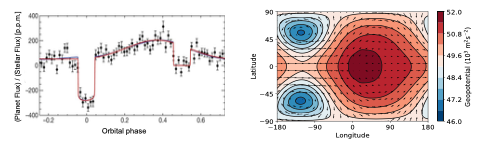
\includegraphics{figures/random-figure.png}
    \caption{Lorem ipsum dolor sit amet, consectetuer adipiscing elit.}
    \label{fig:my_label}
\end{figure}

\section{Acronyms}
Same as above. Entries added into \textbf{frontmatter/acronyms.tex}. An example: the \acrlong{ipcc} can be input in long-form or short-form \acrshort{ipcc}.
\printbibliography[title={References}]
\end{refsection}


% %----------------------------------------------------
% CHAPTER 2: First significant chapter
\begin{refsection}
\chapter{\label{ch2} First significant chapter} 
\begin{mybox}
    \textbf{Abstract} \\
    \small
    \lipsum[1].
\end{mybox}

\section{Introduction}
\label{ch2:intro}
\lipsum[2]
\section{Methods}
\label{ch2:methods}
\lipsum[2]
\section{Results}
\label{ch2:results}


Let's put in a figure.

\begin{figure}[h]
    \centering
    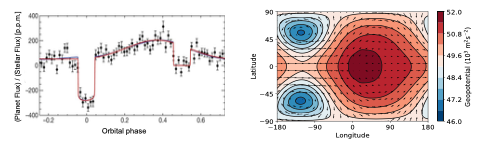
\includegraphics[width=\textwidth]{figures/random-figure.png}
    \caption{Lorem ipsum dolor sit amet, consectetuer adipiscing elit \parencite{Elliott2016}}
    \label{fig:ch2-rand}
\end{figure}

\lipsum[2]
\section{Conclusions}
\label{ch2:conclusions}

\lipsum[2]
\printbibliography[title={References}]
\end{refsection}

% %----------------------------------------------------
% FINAL CHAPTER: THESIS CONCLUSIONS
\begin{refsection}
\chapter{\label{conclusions}Conclusions} 
\lipsum[2]
\printbibliography[title={References}]
\end{refsection}


% % %----------------------------------------------------
% % APPENDIX

% \begin{refsection}
% \chapter{\label{appendix}Appendix} 
% \section{Example calculation 1}
\label{app:calc-1}

Here is an example calculation as shown by \cite{Elliott2016}: \\

\begin{equation}
y = mx + c
\label{eq:cost}
\end{equation} \\
% \printbibliography[title={References}]
% \end{refsection}
% \backmatter

% %----------------------------------------------------
% GLOSSARY
\clearpage
% glossary at the end
\printglossary

\end{document}
